\documentclass[10pt, a4paper]{article}

\usepackage[a4paper, top=0.5cm, bottom=0.5cm, left=0.5cm, right=0.5cm, landscape]{geometry}
\usepackage{mathtools}
\usepackage{amsfonts}
\usepackage{multicol}
\usepackage{setspace}
\usepackage{graphicx}
\usepackage[dvipsnames]{xcolor}
\usepackage{array}



\author{Zachary Chua Yan Ern}
\date{March 2022}
\setstretch{1.25}

\newcommand{\highlight}[1]{{\color{red}\textbf{#1}}}
\newcommand{\blue}[1]{{\color{MidnightBlue}#1}}
\newcommand{\red}[1]{{\color{red}#1}}
\newcommand{\green}[1]{{\color{ForestGreen}#1}}
\newcommand{\header}[1]{{\normalsize\textbf{#1}}}
\newcommand{\tab}[0]{\hspace*{2mm}}

\begin{document}
	\scriptsize %small
	\setlength\parindent{0pt}
	\setlength{\columnseprule}{0.1pt}
	
	\begin{center}
		{\large CS2102 CheatSheet}\\
		by Zachary Chua
	\end{center}

	\begin{multicols*}{3}
		\textbf{Transactions}

		Abstraction for logical unit of work

		\highlight{ACID properties}

		\textbf{Atomicity}: Either all effects of transaction are reflected or none
		
		\textbf{Consistency}: execution of transaction in isolation preserves DB consistency

		\textbf{Isolation}: execution of transaction is isolated from effects of other concurrent transaction executions

		\textbf{Durability}: effects of commited transaction persists even if system failure\\

		\header{Relational Algebra}

		\textbf{Selection: $\sigma _c$}

		$\sigma _c(R)$: selects tuples from relations $R$ that satisfies the \underline{selection condition} $c$

		Result of \underline{comparison operation} involving \highlight{null} is \red{unknown}

		Result of \underline{arithmetic operation} involving \highlight{null} is \highlight{null}

		\textbf{Projection: $\pi _l$}

		$\pi _l$ projects attribute given by a list $l$ of attributes from relation R

		Duplicate records are removed in output relation

		\textbf{Renaming: $\rho _l$}

		$\rho _l$ renames attributes in R based on list of attribute renamings $l$

		$l$: list of attribute renamings $a_i:b_i$ (renames attirbute $a_i$ to $b_i$)\\

		\textbf{Set Operators}

		Set Operators require input relations to be \underline{union compatible}

		Schema of output of R op S is \highlight{identical to schema of R}

		\textbf{Union Compatibility}: 

		\tab 1. have same number of attributes, and

		\tab 2. correesponding attributes have same domains

		Dont't need to have same attribute names

		\textbf{Cross Product, $\times$}: cartesian product

		\textbf{Inner Join, $\Join _c$}		

		$R \Join _c S = \sigma _c(R \times S)$

		Might have to involve renaming attributes if same name

		\textbf{Natural Join, $\Join$}

		$R \Join S = \pi _l(R \Join _c \rho _{a1:b1, \dots, an:bn}(S))$
		where,

		$A$ = common attributes

		$c$ = $(a1 = b1)$ and ... and $(an = bn)$

		$l$ = attributes in A, then attributes in R - A, then attributes in S - A

		natural join removes duplicate columns, joins on attributes w same name
		
		\textbf{Dangling Tuples} - tuple in join operand that does not take part in join operation

		Preserved using \underline{outer joins}

		\textbf{Natural outer joins}: no need state join condition, remove dup column\\

		\header{ER Model}

		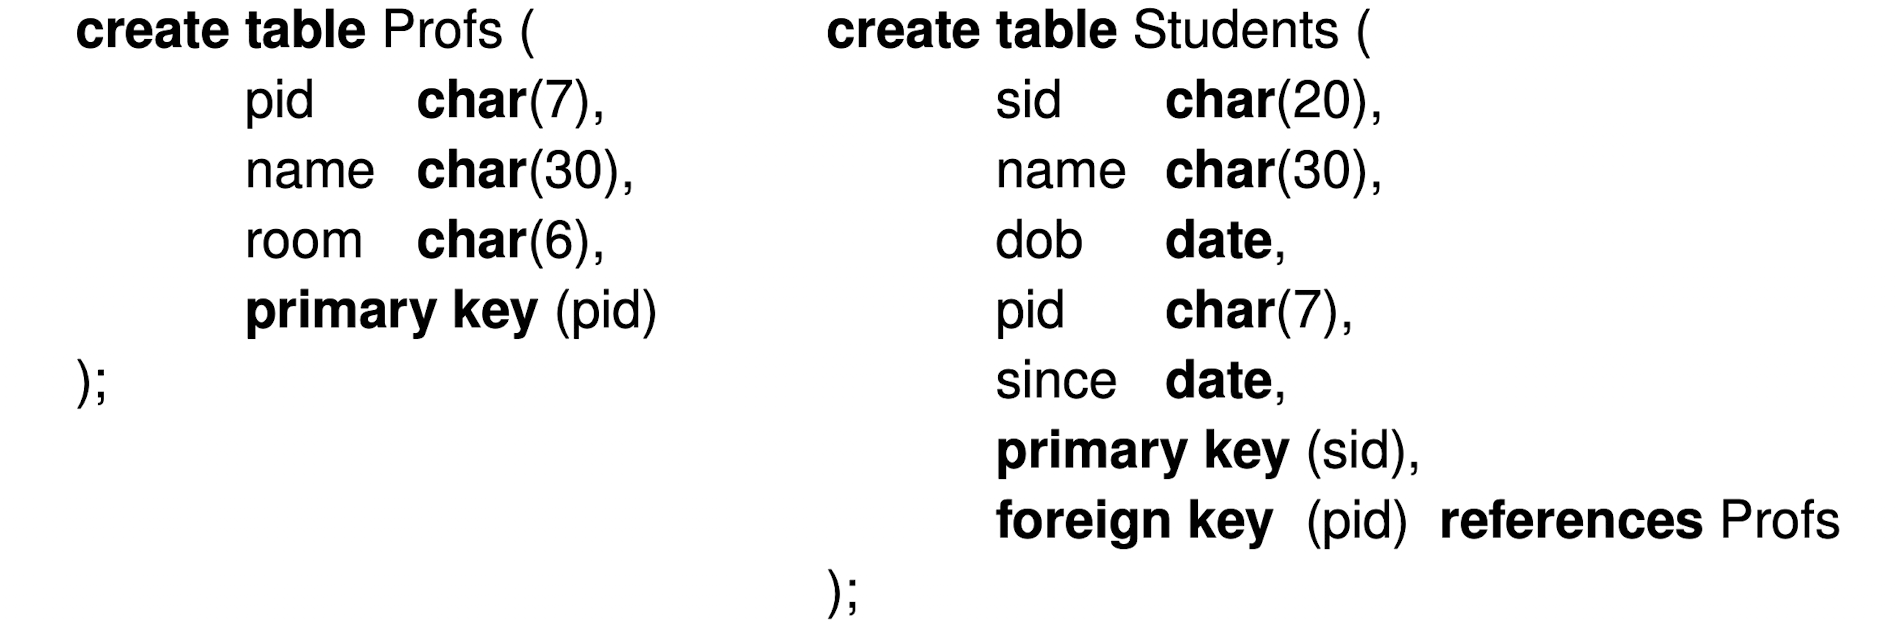
\includegraphics[scale=.23]{./assets/keyConstraint.png}

		Key from Student $\rightarrow$ Supervises (alternative: separate Supervises table)

		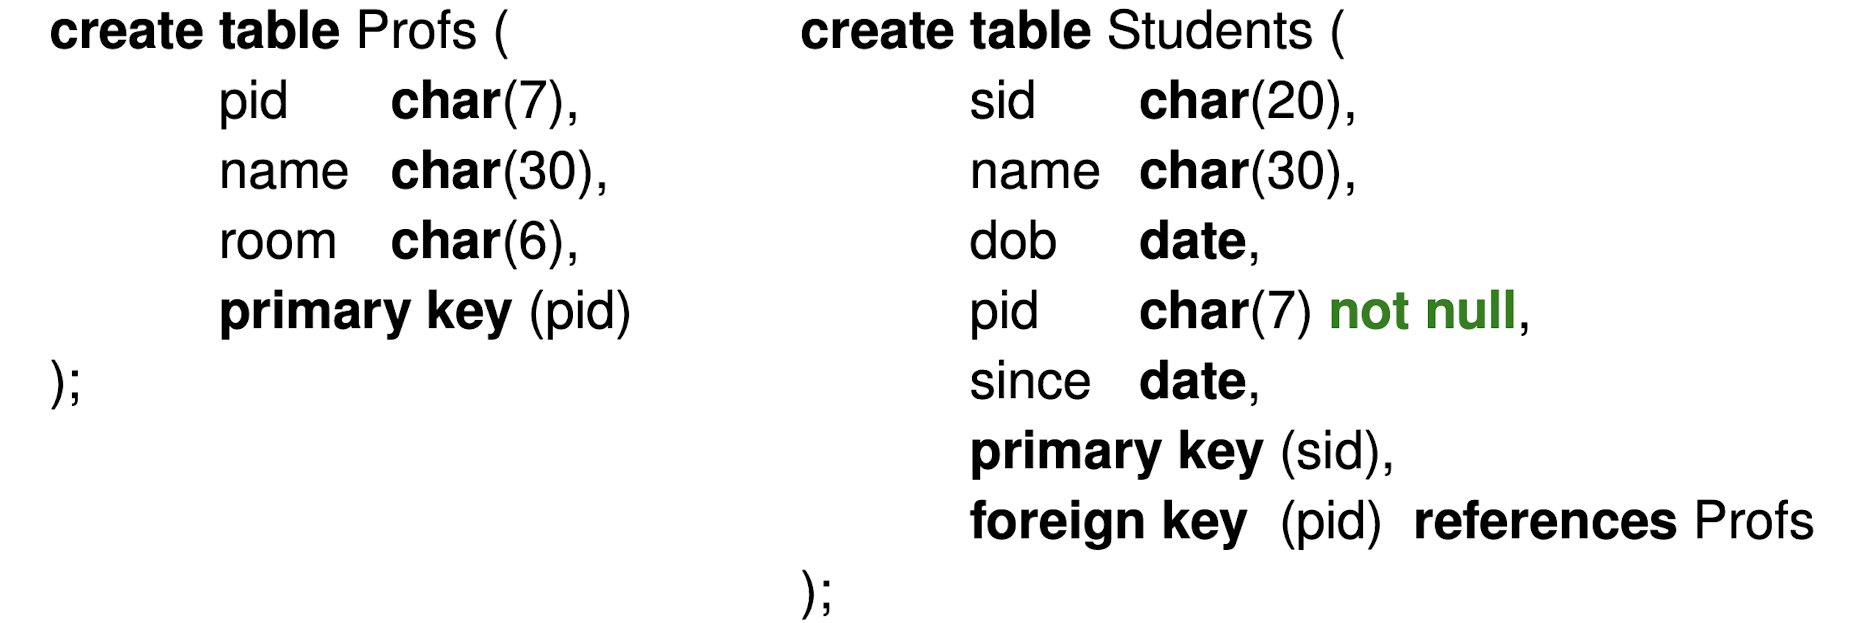
\includegraphics[scale=.23]{./assets/keyAndTotalConstraint.png}
		
		Key and Total Constraint from Students to Supervises R/S

		Separate supervises table needs triggers to enforce Total participation

		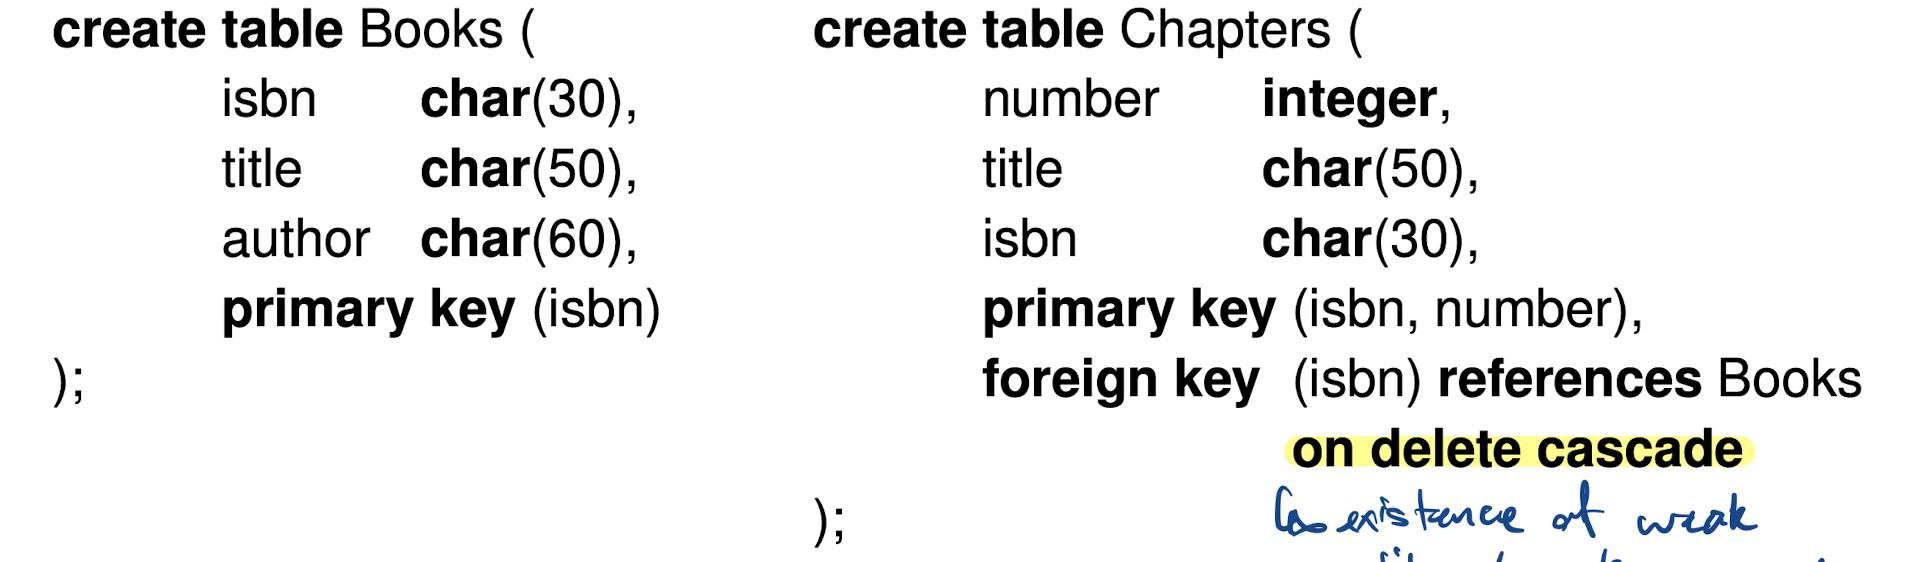
\includegraphics[scale=0.23]{./assets/weakEntity.png}

		Weak Entity Relationship from Chapters to Books

		\textbf{ISA hierarchies}:

		1. Overlap Constraint: Can entity belong to multiple subclasses?

		\tab \textbf{yes}: undirected edge from superclass to triangle, \textbf{no}: Directed edge

		2. Covering Constraint: Does entity have to be one of the subclasses?

		\tab \textbf{yes}: thick edge, \textbf{no}: thin edge\\

		\header{SQL}

		% \textbf{Create/Drop Table}
		% \begin{verbatim}
		% 	create table Students (
		% 	    studentId	integer,
		% 	    name		varchar(100),
		% 	    birthDate	date,
		% 	    dept 		varchar(20)
		% 	);
		% 	drop table Students;
		% 	drop table if exists Students cascade (optional);
		% \end{verbatim}
		% \textbf{Comparison predicates}

		% - Use \texttt{IS NULL} or \texttt{IS NOT NULL} for null values

		% - \texttt{IS DISTINCT FROM} behaviour:

		% \tab - $x <> y$ if both non null

		% \tab - false if both values are null

		% \tab - true if one of the values are null

		% \textbf{Constraints}

		% 1. \texttt{not null}: violated if \texttt{IS NOT NULL} evaluates to false

		% 2. \texttt{unique}: violated if \texttt{x.attr <> y.attr} evaluates to false

		% \tab - nulls allowed because evaluate to \highlight{unknown}

		% 3. \texttt{unique(attr1, attr2)}: \texttt{(x.attr1 <> y.attr1) or (x.attr2 <> y.attr2)}

		% 4. \texttt{primary key}: equivalent to \texttt{unique not null}
		
		% \textbf{Foreign Keys}

		% Syntax: \texttt{foreign key (attr) references Table(column)}

		% \tab - column is PK by default but can also be any unique column(s)

		% \texttt{match full}: does not allow partially null

		% \textbf{Check Constraints}

		% Syntax: \texttt{check(constraint)}

		% named constraint syntax: \texttt{constraint name check (requirement)}

		% \textbf{Insert, Delete, Update}
		% \begin{verbatim}
		% 	-- rest of columns will be null
		% 	insert into Students (name, studentId) 
		% 	values ('Bob', 67890), ('Carol', 11122);
		% 	-- removes all students from Maths Dept
		% 	delete from Students where dept='Maths'; 
		% 	update Accounts 
		% 	set balance = balance + 500
		% 	    name = 'Alice'
		% 	where accountId = 12345;
		% \end{verbatim}

		\textbf{Foreign Key Constraints}

		Delete/ Update tuple may violate FK constraint, specify behaviour

		1. NO ACTION: rejects if violates FK constraint

		2. Restrict: similar to NO ACTION but constraint check cannot be deferred

		3. CASCADE: propagate delete or update to referenced tuple

		4. SET DEFAULT: set to default value (must exist in referenced table)

		5. SET NULL

		Syntax: \texttt{on delete / update cascade}

		% \textbf{Transactions}

		% start with \texttt{begin}, end with \texttt{commit}

		\textbf{Deferrable Constraints}

		Deferrable Constraints: unique, PK, FK

		1. \texttt{deferrable initially deferred}: checked at end of transaction

		2. \texttt{deferrable initially immediate}: checked at end of statement (default)

		% Declaration: 

		% 1. Can declare in schema (under constraint)

		% constraint [constraintName] \dots

		% \tab deferrable initially deferred

		% 2. use \texttt{set constraint}
		
		% begin 

		% set constraints [constraintName] deferred;

		% statements

		% commit\\

		% \textbf{Modifying Schema}
		% \begin{verbatim}
		% 	alter table Students alter column dept drop default;
		% 	alter table Students drop column dept;
		% 	alter table Students add column faculty varchar(20);
		% 	alter table Students add constraint fk_grade foreign key
		% 	(grade) references Grades;
		% \end{verbatim}

		\textbf{Set Operations}

		\texttt{union} $\cup$, \texttt{intersect} $\cap$, \texttt{except} $-$

		\red{Note}: they eliminate duplicate records (to retain use all eg. \texttt{union all})

		\red{Note}: \texttt{intersect} has higher precedence than \texttt{union} and \texttt{except}\\

		\textbf{Subquery Expressions}

		\texttt{exists, in, any / some, all}

		- evaluates inner query for every tuple in table from outer query

		% {\bf \texttt{EXISTS}}

		% Returns \underline{true} if the output of the Subquery is non-empty; \underline{false} ow

		% Opposite is \texttt{NOT EXISTS}

		% {\bf \texttt{IN}}

		% Syntax: \texttt{expression IN (subquery)}

		% Subquery \red{must} return \underline{exactly one} column

		% Returns \underline{false} if the output of the subquery is empty, otherwise result of

		% \centerline{$((v = v_1)$ or \dots or $(v = v_n))$}

		% where v is result of expression and $v_j$ is output of subquery

		% Alternative: \texttt{expression IN (value1, value2, ..., valuen)}

		% {\bf \texttt{ANY / SOME}}

		% Syntax: \texttt{expression op ANY (subquery)}

		% Subquery \red{must} return \underline{exactly one} column

		% Return \underline{false} if subquery output empty or result of 

		% \centerline{$((v$ op $v_i)$ or \dots or $(v$ op $v_n))$}

		% {\bf \texttt{ALL}}

		% Same as \texttt{ANY}, except returns \underline{true} if output of subquery empty, otherwise

		% \centerline{$((v$ op $v_i)$ and \dots and $(v$ op $v_n))$}

		\red{Note}: For \texttt{ALL} if one $v_j$ is \textbf{null} then op evaluates to \textbf{null}, entire result becomes \textbf{null}

		% \textbf{Order by, Limit, Offset}

		% 	\texttt{-- gets the 4th and 5th most expensive pizza}

		% 	\texttt{select pizza, rname, price from Sells order by price desc offset 3 }

		% 	\texttt{limit 2;}

		\textbf{Aggregate Functions} - \texttt{min, max, count, sum, avg}

		Note \texttt{count(A)} counts non-null values in A, \texttt{count(*)} counts rows in table

		\texttt{avg(distinct A)}: average of distinct non null values, \texttt{count(distinct A)}: counts distinct non null values etc

		\highlight{Note}: Aggregate functions can only be used in SELECT, HAVING, ORDER BY (\red{NOT WHERE})

		\texttt{where price = (select max(price) from Sells);} \red{not} where price = max(price)

		{\bf \textbf{GROUP BY}}

		Each output tuple corresponds to one group

		If A in R appearing in SELECT clause, one must hold

		\tab - A in \red{group by}, OR A in \red{aggregated expression} OR \red{grouped by PK}

		\highlight{Note}: if aggregate function in SELECT clause, and \red{no} GROUP BY clause, SELECT clause \red{cannot} contain any column \underline{not in aggregated expression}

		{\bf \texttt{HAVING}}

		\texttt{having} applied to every \red{group}, so attributes in \texttt{HAVING} have same restrictions

		\textbf{Conceptual Evaluation of Queries}

		1. Compute tables in FROM

		2. Select tuples that evaluate to \underline{true} for WHERE

		3. Partition by WHERE

		4. Select groups evaluate to \underline{true} for HAVING

		5. Generate output tuple by selecting attributes in SELECT

		6. Remove duplicate output tuples (if DISTINCT)

		7. Sort by ORDER-by

		8. Remove based on OFFSET and LIMIT

		% \textbf{Conditional Expressions: CASE}
		% \begin{verbatim}
		% 	case 
		% 	    when condition1 then result1
		% 	    ... 
		% 	    when conditionn then resultn 
		% 	    else result0
		% 	end
		% 	    OR
		% 	case expression 
		% 	    when value1 then result1
		% 	    ... 
		% 	    when valuen then resultn
		% 	    else result0
		% 	end
		% \end{verbatim}
		% \textbf{COALESCE}: returns first non-null result in its arguments, or null

		% Syntax: \texttt{coalesce(first, second, third)}

		\textbf{NULLIF}

		Syntax: \texttt{nullif(value1, value2)}

		Returns null if value1 = value2; otherwise returns value1

		\textbf{Universal Quantification}
		\begin{verbatim}
			-- Names of students who have enrolled in all CS Courses
			select name
			from Students S
			where not exists (
			    select courseId
			    from Courses C
			    where dept = 'CS'
			    and not exists (
			        select 1
			        from Enrolls E
			        where E.cid = C.courseId and E.sid = S.studentId
			    )
			);
		\end{verbatim}

		\header{PL/PGSQL}

		\textbf{Functions and Procedures}
		\begin{verbatim}
			CREATE OR REPLACE FUNCTION <name>
			    (IN / OUT <param> <type>, ...)
			RETURNS <type> AS $$
			<code>
			$$ LANGUAGE sql;
			<name>(params);

			CREATE OR REPLACE PROCEDURE <name> 
			    (<param> <type>, ...)
			AS $$ 
			<code>
			$$ LANGUAGE sql;
			CALL <name>(params);
		\end{verbatim}
		Return type (for functions):
		
		- \texttt{VOID}: nothing

		- \texttt{RECORD} or table name: first (one) tuple, if record specify out params

		- \texttt{TABLE(<param> <type>, ...)}: same as \texttt{RECORD}

		\textbf{Control Flow}
		\begin{verbatim}
			If <case> THEN <statement> ;
			ELSIF <case> THEN <statement> ;
			ELSE <statement> ;
			END IF;
			WHILE <condition> LOOP
			    <code>
			END LOOP;
			LOOP
			    EXIT WHEN <condition> ;
				<code>
			END LOOP;
			array INT[] := ARRAY[1,2,3]; -- index starts at 1
			FOREACH d IN ARRAY array LOOP
			    <code>
			END LOOP;
		\end{verbatim}

		\textbf{Cursor}: access each indiv row returned by \texttt{SELECT}

		Declare cursor $\rightarrow$ Open cursor $\rightarrow$ fetch tuple from cursor $\rightarrow$ close cursor

		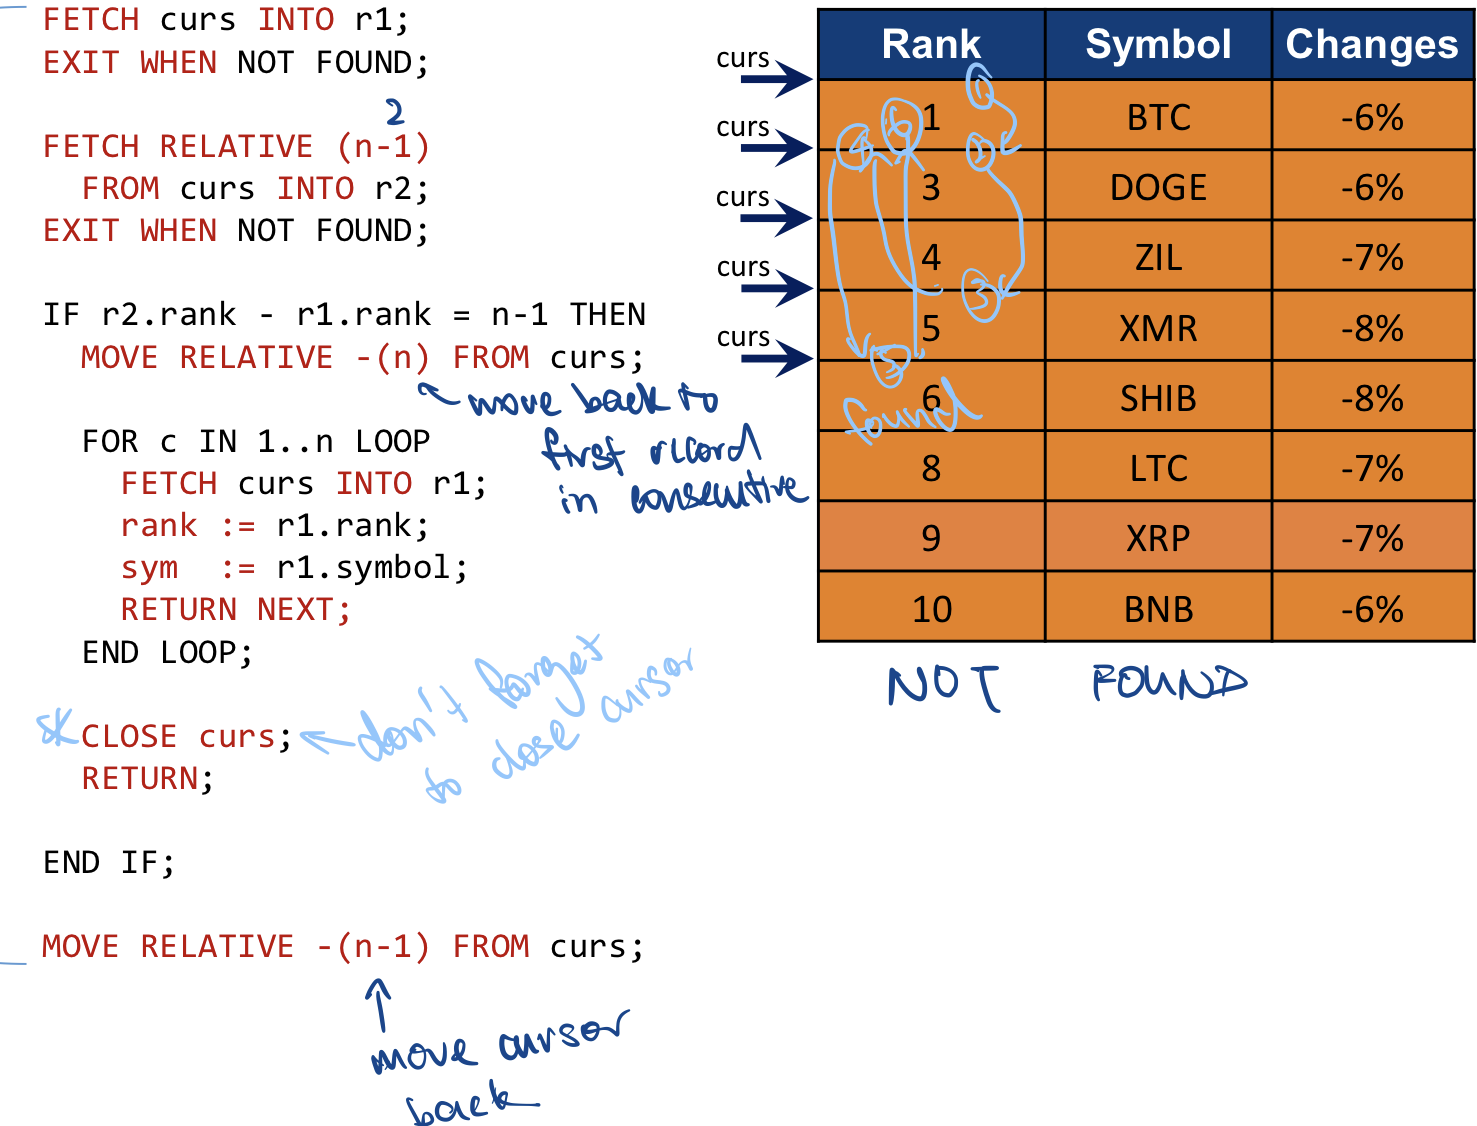
\includegraphics[scale=0.15]{./assets/cursor.png}

		Cursor Movement:

		- \texttt{FETCH curs INTO r;} - fetch then move

		- \texttt{FETCH NEXT FROM curs INTO r;} - move then fetch

		- \texttt{FETCH PRIOR FROM curs INTO r;} 

		- \texttt{FETCH FIRST FROM curs INTO r;} 

		- \texttt{FETCH LAST FROM curs INTO r;} 

		- \texttt{FETCH ABSOLUTE X FROM curs INTO r;} - Fetch Xth tuple

		- \texttt{FETCH RELATIVE X FROM curs INTO r;} 

		- \texttt{MOVE RELATIVE X FROM curs;} - Moves cursor X rows away\\
		
		\header{Triggers}

		\textbf{Trigger Function}
		\begin{verbatim}
			CREATE OR REPLACE FUNCTION <name>() 
			RETURNS TRIGGER AS $$
			BEGIN 
			    <code>
			END;
			$$ LANGUAGE plpgsql;
		\end{verbatim}
		Must return \texttt{TRIGGER} to access:

		\texttt{NEW}: pointer to the tuple to be inserted

		\texttt{OLD}: old tuple being updated / deleted

		\texttt{TG\_OP}, \texttt{TG\_TABLE\_NAME}
		
		% \textbf{Trigger}
		% \begin{verbatim}
		% 	CREATE TRIGGER <name>
		% 	AFTER INSERT (OR DELETE OR UPDATE) ON <table_name>
		% 	FOR EACH ROW EXECUTE FUNCTION <function_name>;
		% \end{verbatim}

		\textbf{Trigger Timing}

		After: Executed after insertion (return value not important)

		Before: Executed before insertion

		Instead Of: function run instead of insertion, can only be \red{defined on views}
		
		\tab - typically used to do something on table instead of on view

		\textbf{Return Value}
		
		BEFORE INSERT: non-null $t$: $t$ is inserted, NULL: nothing inserted  

		BEFORE UPDATE: non-null $t$: $t$ is updated tuple, NULL: no tuple updated

		BEFORE DELETE: non-null $t$: delete (even if $t$ non-existent), NULL: no delete

		\highlight{Note}: Before row-level triggers return \texttt{NULL}, subsequent triggers ignored

		AFTER: return value does not matter

		INSTEAD OF: \texttt{NULL}: ignore rest of operations on row, non null: proceed

		\textbf{Statement Level}

		Return Values: statement level triggers \red{ignore} the values returned by trigger functions

		\red{Note}: RETURN NULL would \red{not} make the database omit the subsequent operations, raise exception to do this

		\highlight{Note}: \texttt{INSTEAD OF} only allowed on row-level, \texttt{BEFORE, AFTER} allowed on both

		\textbf{Deferred Trigger}

		To defer trigger to end of transaction
		\begin{verbatim}
			CREATE CONSTRAINT TRIGGER <name> -- instead of CREATE TRIGGER <name>
			AFTER INSERT OR UPDATE OR DELETE ON <table>
			DEFERRABLE INITIALLY DEFERRED 
			FOR EACH ROW EXECUTE FUNCTION <name>;
		\end{verbatim}
		- \red{Constraint and deferrable together} indicate trigger can be deferred 

		\highlight{NOTE}: Deferred triggers only work with AFTER and FOR EACH ROW

		\textbf{Order of Activation}

		BEFORE statement $\rightarrow$ BEFORE row $\rightarrow$ AFTER row $\rightarrow$ AFTER statement

		Within category, triggers activated in alphabetical order\\

		\header{Functional Dependency}

		Definition: \texttt{$A_1A_2 \dots A_m \rightarrow B_1B_2 \dots B_n$} if 

		1. 2 rows have same values on $A_1, A_2, \dots , A_m$ and

		2. they always have the same values on $B_1, B_2, \dots , B_n$

		If 2 tuples have same NRIC, they have same NAME

		\textbf{Closure}

		1. Initialise the closure to $\{A_1, \dots A_n\}$

		2. If there is an FD: $\{A_1, \dots , A_m\} \rightarrow B$, such that $A_1, \dots , A_m$ are all in closure, then put B into closure

		3. Repeat 2 until no new attributes

		To prove that $X \rightarrow Y$ holds, show that $\{X\}^+$ contains $Y$. Inverse is true

		\textbf{Superkeys, Keys}

		Closure of Superkeys contain all columns in the table

		\red{Note}: if attribute is not in the RHS of any FDs, then must be in key

		\red{Prime Attributes}: attribute that appears in keys\\

		\header{BCNF}

		In BCNF if \red{every non-trivial decomposed} FD has \red{superkey} as its LHS

		\textbf{BCNF check}: No closure violates ``more but not all'' condition
		
		\textbf{BCNF decomposition}: Binary split until subtables are in BCNF

		1. Find subset $X$ of attributes in $R$ that violates ``more but not all''

		2. Decompose $R$ into $R_1$ and $R_2$, such that 

		\tab - $R_1$ contains all attributes in $\{X\}^+$

		\tab - $R_2$ contains all attributes in X and attributes not in $\{X\}^+$

		3. if $R_1$ or $R_2$ not in BCNF, further decompose

		\highlight{NOTE}: BCNF decomposition is not unique, table with \red{2} columns is in BCNF

		\textbf{Projection of FDs}
		
		1. For each attribute subset of $R_i$ derive closure on $R$

		2. Project closure onto $R_i$ by removing attributes not in $R_i$

		\textbf{Lossless decomposition}

		Table decomposed by BCNF can be reconstructed from sub tables.

		BCNF decomposition is lossless because $X$ is key of $R_1$, so for each row in $R_2$ there is a unique row in $R_1$ to join to

		\textbf{Dependency Preservation}: to avoid making ``inappropriate'' updates

		BCNF may not preserve dependencies.

		eg $AB \rightarrow C, B \rightarrow C$, decomposes to $R_1(A, C), R_2(B, C)$, $AB \rightarrow C$ is lost

		$S$ = set of FDs on original table

		$S'$ = set of FDs on decomposed table

		Decomposition \blue{preserves} all FCs iff $S$ and $S'$ are equivalent (use closures)

		\tab - Every FD in $S'$ can be derived from $S$ and vice versa\\ 

		\header{3NF}

		Every non-trivial decomposed FD, LHS superkey, or RHS \red{prime attribute}

		More lenient than BCNF, satisfy BCNF $\rightarrow$ 3NF, converse may not be true

		violate 3NF $\rightarrow$ violate BCNF, converse may not be true

		\textbf{3NF Check}

		``more but not all'', and not all is not prime attribute $\rightarrow$ violate 3NF

		\textbf{3NF decomposition}: n-ary split into tables in 3NF

		1. Derive \red{minimal basis} of S

		2. In minimal Basis, combine FDs with same LHS

		3. Create table for each FD remaining

		4. Make table with Key if none contain key. (To ensure lossless join)

		5. Remove redundant tables

		\textbf{Minimal Basis}: Simplified version of $S$, the set of FDs

		Conditions for minimal basis:

		1. Every FD can be derived from S and vice versa

		2. Every FD is a non-trivial, decomposed FD

		3. No FD in minimal basis is \red{redundant}
		
		4. For each FD in minimal basis, none of the attributes on LHS is \red{redundant}. ie. if remove an attribute from LHS, FD cannot be derived from S

		Algo to find minimal basis:

		1. Decompose FDs

		2. Remove redundant attributes on LHS

		\tab - Remove one, check remaining attributes closure same as before removing.

		\tab eg. remove $A$ from $AB \rightarrow C$, check if $\{B\}^+$ is same as before removing $A$

		3. Remove redundant FDs

		\tab - Remove FD and check if closure of attributes on FD LHS is same

		\tab eg. remove $AB \rightarrow C$, check $\{AB\}^+$ is same as before removing $AB \rightarrow C$

		\highlight{Tip}: $AB \rightarrow C$ is redundant if $B \rightarrow C$ exists











		
	\end{multicols*}

\end{document}	
